\documentclass[]{book}

\usepackage{import}
\usepackage{preamble}
\usepackage{tikz}

\begin{document}

\noindent BECA / Huson / 11.1 IB Math SL \hspace{2in} Name:\\*
31 October 2017
\begin{center}
{\Large Homework: Exponents and radicals}\\
\textit{Do these problems without a calculator. Answer the first page on loose leaf paper.}
\end{center}

%\vspace{0.2 cm}


Simplify, leaving no negative or fractional exponents.

\begin{enumerate}

\item $\displaystyle (\frac{1}{x^{-2}}-4)^2 \times \frac{1}{5}x^{-4} y^{3}$
\item $\displaystyle  \frac{x^2 \sqrt{12x^6}}{xy \sqrt[5]{32x^{-5}}}$
\item $a^3 b^{-3} \div a^{-4} b^{\frac{1}{2}}$
\item $\displaystyle \frac{6}{5} (x^{-2} y)^2 \times \frac{1}{3}(x^4 y^{-1})$
\item $\displaystyle  25^\frac{3}{2}$
\item $\displaystyle  \sqrt[3]{\frac{16a^9 b^{-3}}{z^{-4}}}$

\item $\sqrt{20}$
\item $\sqrt{12x^4}$

\item $4\sqrt{x}-3\sqrt{x}$
\item $\frac{1}{2}\sqrt{ab^2}+\frac{3}{2}b\sqrt{a}$
\item $x^2 \sqrt{xy^3}+3y\sqrt{xy}$

\item $(x^2+x-5)(x-1)$
\item $(2x^2-4x+1)(3x-1)$

\item Let $f(x) = (4x+8)^2 - 3x$ and $g(x)=\frac{1}{2}x-2$. Find $(f \circ g) (x)$\\*[10pt]

Express each item as fractions with rational denominators.
\item $\displaystyle   \frac{1}{\sqrt{2}}$
\item $\displaystyle  \frac{1-x}{\sqrt{x}}$
\item $\displaystyle  \frac{7}{3+\sqrt{5}}$
\item $\displaystyle  \frac{x^2-3}{x-\sqrt{3}}$

\newpage
\item Let $f(x) = x^2 -5x +4$ and $g(x)=x-1$
\begin{enumerate}
    \item Rewrite $f$ in vertex form and state the vertex as an ordered pair.
    \item Factor the function $f$ and write down its roots.
    \item Graph the function $f$, labeling it. Mark the intercepts and graph the axis of symmetry as a dotted line, labeling it with its equation.
    \item Graph $g$ and label it with its name or equation.
    \item Mark the intersections of $f$ and $g$ as ordered pairs. 
    \item Select one of the solutions and show that it satisfies the system by substituting it into both functions.
\end{enumerate}


\begin{figure}[!htbp]
\begin{center}
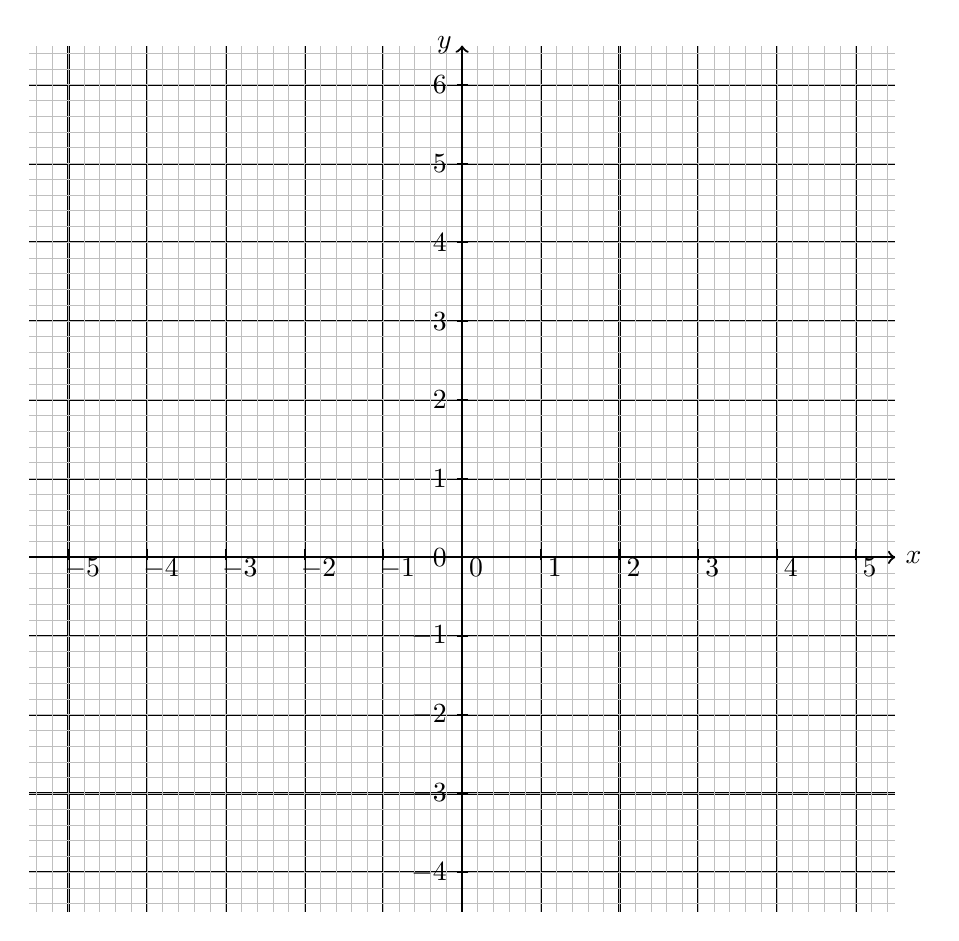
\begin{tikzpicture}

%grid
\draw [thick, color=black,, xstep=1.0cm,ystep=1.0cm] (-5.5,-4.5) grid (5.5,6.5);
\draw [thin, color=lightgray,, xstep=0.2cm,ystep=0.2cm] (-5.5,-4.5) grid (5.5,6.5);

\foreach \x in {-5, -4, -3, -2, -1, 0,1,2,3,4,5}
\draw[shift={(\x,0)},color=black] (0pt,-1pt) -- (0pt,3pt) node[below]  {$\quad \x$};

\foreach \y in {-4, -3, -2,-1,0,1,2,3,4, 5, 6}
\draw[shift={(0,\y)},color=black] (2pt,0pt) -- (-2pt,0pt) node[left]  {$\y$};

\draw [thick, ->] (-5.5,0) -- (+5.5,0) node [right] {$x$};
\draw [thick, ->] (0,-4.5) -- (0,6.5) node [left] {$y$};

%\draw [<-, ->] plot[domain= -1:4] (\x, \x*\x -5*\x +4);
%\draw [<-, ->] plot[domain= -4:5] (\x, \x-1);

\end{tikzpicture}
\end{center}
\end{figure}

\newpage 

\item The function $f(x)=e^x$ is shown on the graph. Sketch $g(x)=f(x-3)$.

\begin{figure}[!htbp]
\begin{center}
\begin{tikzpicture}

%grid
%\draw [thick, color=black,, xstep=1.0cm,ystep=1.0cm] (-5.5,-1.5) grid (5.5,16.5);
%\draw [thin, color=lightgray,, xstep=0.2cm,ystep=0.2cm] (-5.5,-1.5) grid (5.5,16.5);

\foreach \x in {-5, -4, -3, -2, -1, 0,1,2,3,4,5}
\draw[shift={(\x,0)},color=black] (0pt,-3pt) -- (0pt,3pt) node[below]  {$\x$};

\foreach \y in {-1,0,1,2,3,4,5, 6, 7}
\draw[shift={(0,\y)},color=black] (2pt,0pt) -- (-2pt,0pt) node[left]  {$\y$};

\draw [thick, ->] (-5.5,0) -- (+5.5,0) node [right] {$x$};
\draw [thick, ->] (0,-1.0) -- (0,7.5) node [left] {$y$};

\draw [<-, ->] plot[domain= -3:2] (\x, e^\x);

\end{tikzpicture}
\end{center}
\end{figure}

\item The function $f(x)=e^x$ is shown on the graph. Sketch $g(x)=f(-x)+2$. Plot and label the asymptote.

\begin{figure}[!htbp]
\begin{center}
\begin{tikzpicture}

%grid
%\draw [thick, color=black,, xstep=1.0cm,ystep=1.0cm] (-5.5,-1.5) grid (5.5,16.5);
%\draw [thin, color=lightgray,, xstep=0.2cm,ystep=0.2cm] (-5.5,-1.5) grid (5.5,16.5);

\foreach \x in {-5, -4, -3, -2, -1, 0,1,2,3,4,5}
\draw[shift={(\x,0)},color=black] (0pt,-3pt) -- (0pt,3pt) node[below]  {$\x$};

\foreach \y in {-1,0,1,2,3,4,5, 6, 7}
\draw[shift={(0,\y)},color=black] (2pt,0pt) -- (-2pt,0pt) node[left]  {$\y$};

\draw [thick, ->] (-5.5,0) -- (+5.5,0) node [right] {$x$};
\draw [thick, ->] (0,-1.0) -- (0,7.5) node [left] {$y$};

\draw [<-, ->] plot[domain= -3:2] (\x, e^\x);

\end{tikzpicture}
\end{center}
\end{figure}

\newpage
\item Graph the function $f(x) = x^2 - 4$ over the domain $x \geq 0$ on the grid below. 
\begin{enumerate}
    \item Label the $y$-intercept as an ordered pair.
    \item Label the point representing the solution to the equation $f(x)=0$ as an ordered pair.\\*[25pt]
    \item Write down the value of $f^{-1}(-3)$ and label the point $(f^{-1}(-3), -3)$.\\*[25pt]
    \item Graph the inverse function, $f^{-1}(x)$.\\*[15pt]
\end{enumerate}

\begin{figure}[!htbp]
\begin{center}
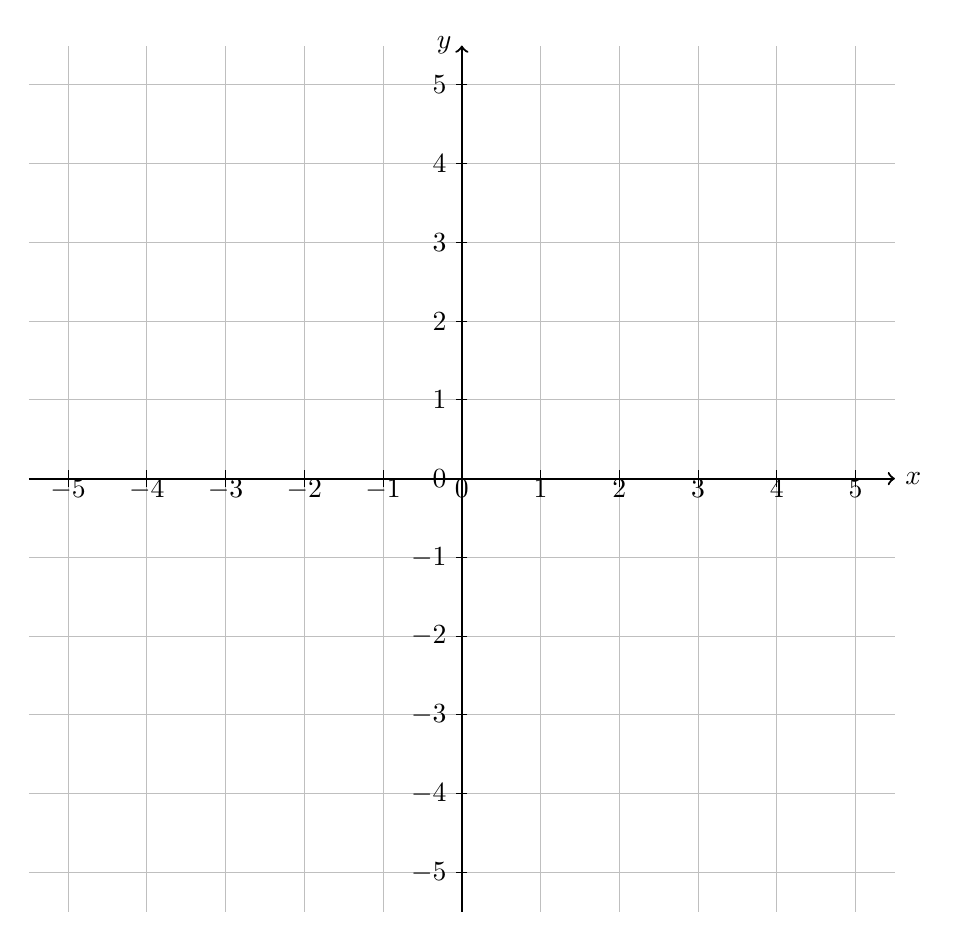
\begin{tikzpicture}

%grid
\draw [thin, color=lightgray,, xstep=1.0cm,ystep=1.0cm] (-5.5,-5.5) grid (5.5,5.5);
%\draw [thin, color=lightgray,, xstep=0.2cm,ystep=0.2cm] (-5.5,-1.5) grid (5.5,16.5);

\foreach \x in {-5, -4, -3, -2, -1, 0,1,2,3,4,5}
\draw[shift={(\x,0)},color=black] (0pt,-3pt) -- (0pt,3pt) node[below]  {$\x$};

\foreach \y in {-5, -4, -3, -2, -1, 0,1,2,3,4,5}
\draw[shift={(0,\y)},color=black] (2pt,0pt) -- (-2pt,0pt) node[left]  {$\y$};

\draw [thick, ->] (-5.5,0) -- (+5.5,0) node [right] {$x$};
\draw [thick, ->] (0,-5.5) -- (0,5.5) node [left] {$y$};

%\draw plot[domain= 0:3] (\x, \x*\x - 4);

\end{tikzpicture}
\end{center}
\end{figure}



\end{enumerate}

\end{document}